% Active Coupling Discovery via Coordinated Perturbation in Autonomous Optimizers
% Detection Paper — Paper 1
%
% Co-authored-by: cherusk <10729954+cherusk@users.noreply.github.com>

\documentclass[11pt,a4paper]{article}

% ── Encoding & Fonts ──────────────────────────────────────────────
\usepackage[utf8]{inputenc}
\usepackage[T1]{fontenc}
\usepackage{libertine}
\usepackage[libertine]{newtxmath}

% ── Math ──────────────────────────────────────────────────────────
\usepackage{amsmath}
\let\Bbbk\relax
\usepackage{amssymb}
\let\openbox\relax
\usepackage{amsthm}

% ── Graphics & Figures ────────────────────────────────────────────
\usepackage{graphicx}
\usepackage{booktabs}
\usepackage{subcaption}
\usepackage{pgfplots}
\pgfplotsset{compat=1.16}
\usepackage{tikz}
\usetikzlibrary{positioning, arrows.meta, shapes.geometric, calc, fit}

% ── Layout ────────────────────────────────────────────────────────
\usepackage[margin=2cm]{geometry}
\usepackage{setspace}
\setstretch{1.1}
\usepackage{microtype}
\usepackage{titlesec}
\usepackage{parskip}

% ── Section formatting ────────────────────────────────────────────
\titleformat{\section}{\large\bfseries}{\thesection}{0.5em}{}
\titleformat{\subsection}{\normalsize\bfseries}{\thesubsection}{0.5em}{}
\titleformat{\subsubsection}{\normalsize\itshape}{\thesubsubsection}{0.5em}{}
\titlespacing*{\section}{0pt}{1.5ex plus 0.5ex minus 0.2ex}{0.8ex}
\titlespacing*{\subsection}{0pt}{1.2ex plus 0.3ex}{0.5ex}

% ── References ────────────────────────────────────────────────────
\usepackage[numbers,sort&compress,square]{natbib}
\bibliographystyle{abbrvnat}

% ── Links ─────────────────────────────────────────────────────────
\usepackage[hidelinks]{hyperref}

% ── Listings ──────────────────────────────────────────────────────
\usepackage{listings}

% ── Title ─────────────────────────────────────────────────────────
\title{The Impulse Protocol: Non-Destructive Coupling \\
       Discovery in Autonomous Agents}
\author{
  Matthias Tafelmeier \\
  Independent Scientist \\
  Hof, Germany \\
  \href{https://orcid.org/0009-0005-7399-5584}{ORCID: 0009-0005-7399-5584}
}
\date{}

\begin{document}
\maketitle

\begin{abstract}
Multiple autonomous agents tending a shared substrate---physical,
computational, or mathematical---unknowingly affect each other through coupling channels
invisible to each agent individually. We present the impulse protocol,
a method by which
such agents discover their coupling structure through coordinated
perturbation: one agent deliberately drives its parameters
to extremes (push), then returns to neutral (pause), while all others
hold fixed as passive sensors. An adaptive perturbation calibration
phase finds a safe amplitude before each push block. A
constant-false-alarm-rate (CFAR) step-change detector then evaluates
whether each receiver's signal exhibits a reversible shift
correlated with the sender's perturbation.

The protocol is coupling-shape-agnostic---it does not model the
coupling function and detects linear, threshold, polynomial, and
saturated coupling equally. We characterize the method empirically
on a synthetic bench with planted ground truth, sweeping coupling
strength ($0.1$--$0.9$), noise level ($\sigma = 0.01$--$0.20$), and
coupling shape. The detection floor lies between coupling $0.1$ and
$0.2$ at noise $\sigma = 0.02$, with measured step amplitudes within
$5\%$ of planted ground truth. Zero false positives were observed
across all noise levels tested.

The contribution is the protocol that makes coupling
\emph{detectable}---not a novel detector. The detection backend is
pluggable. The key insight is that autonomous agents, unaware of each
other and communicating only through the substrate they tend, can be
coordinated to take turns as active perturbers and passive observers
through a shared lease---transforming an unresolvable observational
confound into a structured experiment.
\end{abstract}

\noindent\textbf{Keywords:} active probing, coupling discovery, autonomous agents, impulse protocol, CFAR detection, multi-agent coordination, non-destructive perturbation, cybernetics

% ── Body ──────────────────────────────────────────────────────────
\section{Introduction}
\label{sec:introduction}

Complex coupled systems---data centers, microgrids, process plants,
distributed databases, microservice architectures, compiler
pipelines---share a fundamental problem: their internal coupling
structure is hidden. Which subsystems affect which others,
through which channels, at what strength? The design documentation
specifies intended interfaces, but operational reality includes
emergent coupling paths created by the shared substrate that no
blueprint captures and no expert enumerates~\citep{ljung1999sid}.

Three existing approaches all fail to discover this structure in live
systems. Analytical modeling requires knowing the system's structure
a priori. Statistical observation---cross-correlation, Granger
causality, transfer entropy---cannot separate causal coupling from
co-movement when both subsystems are actively adjusting, because the
dominant noise source is the agents' own
exploration~\citep{sugihara2012ccm, runge2018confounding}. Expert
systems capture design intent, not operational reality, and go stale
as the system drifts.

\paragraph{The confounding problem.}
Consider multiple autonomous agents, each independently tending a
portion of a shared substrate. Each agent adjusts its own parameters
toward its own objective. The agents are unaware of each other.
Yet they communicate involuntarily through the substrate: when one
agent changes its parameters, the system responds in ways
that shift other agents' readings.

When all agents are actively tending, their objective readings move
for two confounded reasons: their own parameter changes and the other
agents' influence. No passive observer can separate these
contributions. The confounding is structural, not statistical---no
amount of observational data resolves it without intervention. This
is why cross-correlation, Granger causality, and transfer entropy all
fail on actively explored systems. They cannot distinguish ``shifting
together because coupled'' from ``shifting together because each is
independently adjusting.''

\paragraph{The key insight.}
The confound disappears if one agent stops exploring and holds still
while another perturbs. With the receiver frozen, any change in its
signal is attributable to the sender's perturbation---not to its own
adjustments. The agent ceases to be an explorer and becomes a
sensor. The sender ceases to explore and becomes a stimulus.

This is the active probing paradigm, borrowed from radar and
seismology: inject a known signal into the medium and observe the
response. The system describes itself through its response to
perturbation, rather than through passive observation of its
behavior. The coupling graph is not inferred from correlations---it
is measured as a set of impulse responses.

\paragraph{Our approach.}
We embed this paradigm inside the agents' normal operation through a
coordinated push/pause/hold protocol. The protocol directs the agents
to take turns: one agent (the sender) drives its parameters to
extremes, then returns to neutral, while all others hold fixed as
passive sensors. An adaptive calibration phase finds a safe
perturbation amplitude before each push block, backing off
exponentially if the system destabilizes. A constant-false-alarm-rate
(CFAR) step-change detector evaluates whether each receiver's signal
exhibits a reversible shift---rising during push, recovering during
pause. The ABA block design eliminates drift confounds: a monotonic
trend produces a rising edge but not a falling edge.

The protocol requires no information exchange beyond scheduling
(``whose turn is it''), enforced through a shared lease with fencing
tokens. Agents do not share objectives, results, or detected edges.
Each discovers coupling purely by watching its own signal shift when
another agent perturbs the substrate.

\paragraph{Coupling-shape agnosticism.}
Because the protocol measures step response---not frequency response,
not correlation structure---it is agnostic to the coupling function's
shape. Linear coupling produces a proportional step. Threshold
coupling produces a discontinuous jump. Saturation coupling produces
a compressed or inverted step. Polynomial coupling produces a
quadratic step. The detector asks only: did the signal change and
recover? The shape of the response determines the step amplitude but
not whether coupling exists.

\paragraph{Contributions.}
\begin{enumerate}
  \item A coordination protocol---push, pause, hold, with adaptive
    perturbation calibration and turn-taking through a fencing-token
    lease---that enables autonomous agents to discover coupling
    structure through their shared substrate without exchanging
    information beyond scheduling.
  \item Empirical characterization on a synthetic bench with planted
    ground truth across four coupling shapes (linear, threshold,
    saturation, polynomial), five noise levels, and six coupling
    strengths. Detection floor, noise boundary, and false positive
    rate are measured and reported honestly.
  \item Step amplitude measurements within 5\% of ground truth across
    the detectable range, with zero false positives across all noise
    levels tested.
\end{enumerate}

The contribution is the protocol that makes coupling
\emph{detectable}---not a novel detector. CFAR is established
technology from radar signal processing~\citep{finn1968cfar}. What
is new is the choreography: autonomous agents, unaware of each other
and communicating only through the substrate they tend, taking turns
as active perturbers and passive observers. The agent that was
exploring blindly becomes a measurement instrument. The probe
\emph{is} the experiment.

\section{Related Work}
\label{sec:related}

The push/pause/hold protocol draws on active-probing paradigms from
several fields where injecting a known signal into a medium and
observing the response is the standard approach to discovering
hidden structure.

\paragraph{Radar and sonar.}
Constant-false-alarm-rate detection was developed for radar signal
processing~\citep{finn1968cfar}. A transmitter emits a known waveform;
a receiver listens for echoes. The CFAR threshold adapts to local
noise conditions, maintaining a constant false-alarm probability
regardless of background noise level. Active sonar applies the same
principle underwater: a sound pulse propagates through the medium, and
the return signal reveals structure (seafloor, submarines, fish
schools) that passive listening cannot detect. Our protocol applies
this paradigm to coupled systems: the push is the transmitted pulse,
the receiver's objective is the return signal, and CFAR discriminates
the coupling step from intrinsic noise.

\paragraph{Seismology.}
Controlled-source seismology detonates explosives or vibrates the
ground at known locations, then measures ground motion at distant
sensors. The subsurface structure---rock layers, fault lines, fluid
reservoirs---is inferred from how the seismic waves propagate and
reflect. The structure cannot be observed passively; it must be
excited. Our method follows the same logic: coupling structure is
inferred from how a perturbation propagates from one agent to
another through the substrate.

\paragraph{Functional brain imaging (fMRI).}
In functional MRI, researchers study brain activity by presenting
controlled stimuli and measuring the hemodynamic response---the
slow, sustained blood-oxygen change that follows neural activation.
The hemodynamic response function (HRF) is a low-pass filter that
smears brief neural events into sustained signal changes. This led
to the \emph{block design} paradigm~\citep{friston1999fmri}:
sustained stimulation blocks of 20--30 seconds alternating with rest
periods, rather than single brief events. Our push/pause blocks are
the same design: a sustained perturbation block that survives the
substrate's thermal mass or response latency, followed by a pause
block that captures recovery. The ABA structure (stimulus, rest,
stimulus) is standard practice in experimental psychology and
neuroscience~\citep{box1978statistics}.

\paragraph{Medical percussion.}
The oldest active-probing diagnostic: a physician taps the body and
listens to the resonance. Solid tissue, fluid-filled cavities, and
air-filled spaces produce different sounds. The technique dates to
the 18th century~\citep{auerbrugger1761percussion}. The principle---
perturb the system, listen to the response, infer internal
structure---is exactly ours, applied to coupling channels between
autonomous agents.

\paragraph{Causal discovery.}
Pearl's do-calculus~\citep{pearl2009causality} provides the
theoretical framework for causal inference from interventions.
Convergent cross-mapping~\citep{sugihara2012ccm} infers coupling
from time series but fails when systems are actively exploring.
Neural relational inference~\citep{kipf2018nri} learns interaction
graphs from trajectories but operates passively. Our method differs
in that the interventions are performed by autonomous agents on
themselves, coordinated through a shared lease, rather than by a
central researcher.

\paragraph{Network tomography.}
Network tomography~\citep{vardi1996tomography} infers internal
network properties from end-to-end measurements using active probe
packets. Active topology inference~\citep{coates2002tomography}
selects measurement paths adaptively to reduce uncertainty about
network structure. These approaches share our active-probing
philosophy but assume a single centralized prober with an explicit
identification objective. Our agents are autonomous---each with its
own objective---and the probing is a cooperative side effect of
coordination, not the agents' primary goal.

\section{Method}
\label{sec:method}

\subsection{System Model}

We consider $N$ autonomous agents (\emph{tenders}), each tending a
portion of a shared substrate. Agent $i$ has a parameter vector
$\mathbf{p}_i \in \mathbb{R}^{d_i}$ and an objective function $f_i$
toward an objective. The substrate couples the agents: agent
$i$'s objective reading depends not only on its own parameters but
also on other agents' parameters through hidden coupling channels:
\begin{equation}
  f_i(\mathbf{p}_i, \mathbf{p}_{j \neq i}) = g_i(\mathbf{p}_i) +
    \sum_{j \neq i} c_{ji}(\mathbf{p}_j)
\end{equation}
where $g_i$ is the agent's own response and $c_{ji}$ is the coupling
contribution from agent $j$ to agent $i$. The coupling function
$c_{ji}$ may be linear, nonlinear, or discontinuous. The coupling
structure---which agents affect which, through which channels, at
what strength---is unknown. Discovering it is the goal.

\subsection{Agent Operation}

Each agent runs a continuous trial loop. In normal operation, the
agent samples a parameter vector via a metaheuristic search
strategy (e.g., TPE, CMA-ES, NSGA-II), applies it to the substrate, reads back
its objective, and records the result. This is the \texttt{OPTIMIZE}
state---the agent's default behavior.

The coordination protocol interrupts this loop periodically to run
detection rounds. Crucially, the perturbations during detection
operate on the \emph{same parameters} the agent controls during
normal operation---the same knobs, within the same defined bounds.
Safety is actively enforced through guardrails: per-trial checks on
objective values and system state that reject configurations
exceeding safe operating limits. The IMPULSE\_CALIB phase probes at
decreasing scale and backs off immediately on any guardrail
violation. Only an amplitude that passes all guardrails is locked
for the push block.

The protocol does not inject faults, disrupt services, or push the
system outside its operating envelope. It adjusts known control
parameters to the edge of their range, observes the response, and
returns to neutral. The system continues operating throughout;
detection is non-destructive. This distinguishes the approach from
chaos engineering or fault injection, which deliberately break
components to test resilience.

\subsection{The Impulse Protocol}

\subsubsection{Sender State Machine}

A detection round for the sender consists of eight states:

\begin{enumerate}
  \item \textbf{\texttt{OPTIMIZE}}: Normal parameter exploration. After
    a minimum number of completed trials ($\geq 15$) and at least two
    active agents, the agent attempts to acquire the sender lease.

  \item \textbf{\texttt{HOLD\_CALIB}}: The sender establishes neutral
    hold parameters---values where its own objective is stable and the
    system is alive. When hold parameters are provided in
    configuration, this step is immediate. Otherwise, the sender
    searches for flat parameters by sampling its objective at
    candidate neutral values and accepting when the standard deviation
    falls below a threshold ($\sigma < 0.05$).

  \item \textbf{\texttt{IMPULSE\_CALIB}}: The sender probes at
    decreasing perturbation scale to find a safe amplitude. Starting
    at full scale ($1.0$), it drives its top-3 parameters (by range)
    toward their upper bounds. If guardrails are violated (e.g., the
    system destabilizes), it backs off: $1.0 \to 0.5 \to 0.25 \to
    0.125$. The first scale that passes becomes the locked amplitude
    for the entire push block. This adaptive calibration ensures the
    perturbation is large enough to produce a detectable signal but
    not so large as to harm the live system.

  \item \textbf{\texttt{PUSH}}: The sender perturbs at the locked
    scale for $B_{\text{push}}$ consecutive trials. Each trial applies
    the extreme parameters, reads back, and records the objective.
    The coupling signal propagates through the substrate to any
    coupled receivers.

  \item \textbf{\texttt{PAUSE}}: The sender returns to neutral hold
    parameters for $B_{\text{pause}}$ consecutive trials. This is the
    ABA recovery---the coupling signal should revert. The receiver's
    signal during this window serves as the post-intervention
    baseline.

  \item \textbf{\texttt{DONE}}: The sender releases the lease and
    clears coordination state.

  \item \textbf{\texttt{COOLDOWN}}: The sender waits a short period
    (5 trials) before re-acquiring, giving other agents a chance to
    take their turn. This enforces fairness in turn-taking.

  \item \textbf{\texttt{HOLD}} (receiver): While any sender holds the
    lease, all other agents enter HOLD---fixing their parameters at
    neutral values and acting as passive sensors. Each hold trial is
    tagged with the sender's current lease phase, so the detector
    can later segment receiver observations into push-window and
    pause-window samples.
\end{enumerate}

\subsubsection{Lease and Turn-Taking}

Only one agent may be sender at any time. A shared lease
(row in a coordination database) enforces this. The lease uses:

\begin{description}
  \item[Fencing tokens] A monotonically increasing token is written
    on each lease acquisition. Every lease mutation (heartbeat,
    budget decrement, release) is guarded by a \texttt{WHERE token =
    $t$} check. If another agent steals the lease (via stale
    recovery), the old sender's token no longer matches and its
    writes are silently rejected---preventing split-brain.
  \item[Count-based budget] The lease tracks
    \texttt{push\_remaining} and \texttt{pause\_remaining} counters
    rather than wall-clock expiry. The sender's turn lasts exactly
    as long as it has budget, avoiding premature expiry when trials
    run slowly (database retries, slow effectuation).
  \item[Heartbeat staleness] A crashed sender's lease is recovered
    when its heartbeat exceeds $5 \times$ the worst-case trial
    duration. Budget alone is insufficient because a crashed sender's
    counters stay positive forever.
\end{description}

\begin{figure*}[t]
\centering
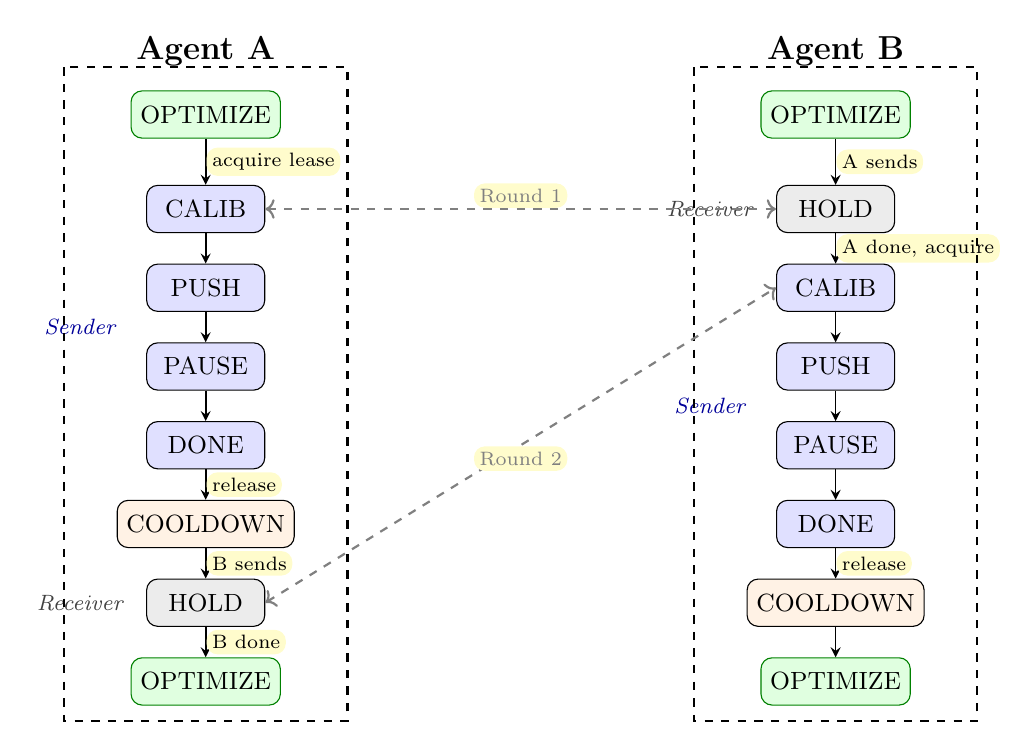
\begin{tikzpicture}[
  node distance=1.0cm,
  st/.style={rectangle, draw, rounded corners, minimum width=1.5cm, minimum height=0.6cm, font=\small},
  send/.style={st, fill=blue!12},
  recv/.style={st, fill=gray!15},
  shared/.style={st, fill=green!12, draw=green!50!black},
  cooldown/.style={st, fill=orange!10},
  arrow/.style={->, >=stealth, semithick},
  tlabel/.style={font=\scriptsize, fill=yellow!20, rounded corners, inner sep=2pt},
]

% ══ Column positions ══
\def\xa{0}
\def\xb{8}

% ══ Agent A (left) ══
\node[font=\large\bfseries] at (\xa, 1.0) {Agent A};

\node[shared] (aopt0) at (\xa, 0.2) {OPTIMIZE};
\node[send] (acalib) at (\xa, -1.0) {CALIB};
\node[send] (apush) at (\xa, -2.0) {PUSH};
\node[send] (apause) at (\xa, -3.0) {PAUSE};
\node[send] (adone) at (\xa, -4.0) {DONE};
\node[cooldown] (acool) at (\xa, -5.0) {COOLDOWN};
\node[recv] (ahold) at (\xa, -6.0) {HOLD};
\node[shared] (aopt1) at (\xa, -7.0) {OPTIMIZE};

\draw[arrow] (aopt0) -- node[tlabel, right] {acquire lease} (acalib);
\draw[arrow] (acalib) -- (apush);
\draw[arrow] (apush) -- (apause);
\draw[arrow] (apause) -- (adone);
\draw[arrow] (adone) -- node[tlabel, right] {release} (acool);
\draw[arrow] (acool) -- node[tlabel, right] {B sends} (ahold);
\draw[arrow] (ahold) -- node[tlabel, right] {B done} (aopt1);

% Sender/Receiver labels
\node[font=\footnotesize\itshape, blue!60!black] at (\xa-1.6, -2.5) {Sender};
\node[font=\footnotesize\itshape, gray!50!black] at (\xa-1.6, -6.0) {Receiver};

% Agent A box
\draw[dashed, thick] (\xa-1.8, 0.8) rectangle (\xa+1.8, -7.5);

% ══ Agent B (right) ══
\node[font=\large\bfseries] at (\xb, 1.0) {Agent B};

\node[shared] (bopt0) at (\xb, 0.2) {OPTIMIZE};
\node[recv] (bhold) at (\xb, -1.0) {HOLD};
\node[send] (bcalib) at (\xb, -2.0) {CALIB};
\node[send] (bpush) at (\xb, -3.0) {PUSH};
\node[send] (bpause) at (\xb, -4.0) {PAUSE};
\node[send] (bdone) at (\xb, -5.0) {DONE};
\node[cooldown] (bcool) at (\xb, -6.0) {COOLDOWN};
\node[shared] (bopt1) at (\xb, -7.0) {OPTIMIZE};

\draw[arrow] (bopt0) -- node[tlabel, right] {A sends} (bhold);
\draw[arrow] (bhold) -- node[tlabel, right] {A done, acquire} (bcalib);
\draw[arrow] (bcalib) -- (bpush);
\draw[arrow] (bpush) -- (bpause);
\draw[arrow] (bpause) -- (bdone);
\draw[arrow] (bdone) -- node[tlabel, right] {release} (bcool);
\draw[arrow] (bcool) -- (bopt1);

% Sender/Receiver labels
\node[font=\footnotesize\itshape, gray!50!black] at (\xb-1.6, -1.0) {Receiver};
\node[font=\footnotesize\itshape, blue!60!black] at (\xb-1.6, -3.5) {Sender};

% Agent B box (same size as A)
\draw[dashed, thick] (\xb-1.8, 0.8) rectangle (\xb+1.8, -7.5);

% ══ Lease coordination ══
% Round 1: A enters CALIB (holds lease), B observes and enters HOLD
\draw[dashed, gray, thick, <->] (acalib.east) -- node[tlabel, above] {Round 1} (bhold.west);

% Round 2: B enters CALIB (holds lease), A observes and enters HOLD
\draw[dashed, gray, thick, <->] (ahold.east) -- node[tlabel, below] {Round 2} (bcalib.west);

\end{tikzpicture}
\caption{Two-agent turn-taking in the impulse protocol. Both agents
start in OPTIMIZE. In Round 1, Agent A acquires the sender lease and
enters the detection cycle: CALIB (hold neutral, find safe perturbation
amplitude), PUSH (drive parameters to extremes), PAUSE (return to
neutral), DONE (release lease). Agent B observes the active lease
and enters HOLD as passive receiver throughout A's detection cycle.
After cooldown, the roles reverse for Round 2. CALIB encompasses
HOLD-CALIB (parameter flatness search) and IMPULSE-CALIB (adaptive
perturbation with guardrail backoff). Dashed arrows show lease
pairing: while one agent holds the sender lease, the partner is in
HOLD.}
\label{fig:state-machine}
\end{figure*}


\subsection{CFAR Step-Change Detection}

After rounds complete, the detector evaluates each ordered
sender--receiver pair. For each pair, the receiver's hold-trial
objectives are segmented by the sender's push/pause timestamps into:

\begin{itemize}
  \item \emph{Baseline window}: receiver values during the sender's
    pause phase (post-intervention recovery)
  \item \emph{Push window}: receiver values during the sender's push
    phase
\end{itemize}

A noise-adaptive threshold is computed from the baseline:
\begin{equation}
  T = k \cdot \widehat{\sigma}_{\text{baseline}}, \quad
  k = N_{\text{ref}} \left( P_{\text{fa}}^{-1/N_{\text{ref}}} - 1 \right)
  \label{eq:threshold}
\end{equation}
where $\widehat{\sigma}$ is the scaled median absolute deviation
(MAD $\times$ 1.4826, a robust $\sigma$-estimator), $N_{\text{ref}}$
is the number of baseline samples, and $P_{\text{fa}} = 0.05$.

A round is \emph{detected} if both:
\begin{align}
  |\text{push\_median} - \text{baseline\_median}| &\geq T \label{eq:rising} \\
  |\text{push\_median} - \text{pause\_median}| &\geq T \label{eq:falling}
\end{align}

Condition~(\ref{eq:rising}) detects the step; condition~(\ref{eq:falling})
enforces reversibility. A monotonic drift would satisfy
(\ref{eq:rising}) but fail (\ref{eq:falling}) because the pause-phase
values would not revert to baseline.

\subsection{Observation Parameters}
\label{sec:obs-params}

All experiments use the following parameters unless otherwise stated:

\begin{center}
\begin{tabular}{ll}
  \toprule
  Parameter & Value \\
  \midrule
  Push block size ($B_{\text{push}}$) & 15 trials \\
  Pause block size ($B_{\text{pause}}$) & 15 trials \\
  Min.\ exploration before detection & 15 trials \\
  Cooldown (turn-taking fairness) & 5 trials \\
  Impulse calibration scales & $1.0, 0.5, 0.25, 0.125$ \\
  Hold parameters & midpoint ($50, 50, 50$) \\
  Push target & top-3 params $\to$ upper bound \\
  CFAR $P_{\text{fa}}$ & 0.05 \\
  Min.\ reference cells (baseline) & 3 \\
  Min.\ test cells (push/pause) & 3 \\
  \bottomrule
\end{tabular}
\end{center}

Detection boundaries are parameterized by observation budget.
Increasing block sizes or the number of rounds lowers the boundary,
as the CFAR scale factor $k$ decreases with more reference cells.
The impulse calibration adapts perturbation amplitude to system
constraints---this parameter is not fixed but discovered per system.

\section{Experiments}
\label{sec:experiments}

\subsection{Synthetic Bench}

We validate on a configurable synthetic bench
(\texttt{bench-generic}) with planted ground-truth coupling. The
bench hosts multiple virtual nodes in a single container, each
exposed via HTTP. A topology file specifies:

\begin{itemize}
  \item Node parameters (count, bounds, objective weights)
  \item Directed edges with coupling strength and channel
  \item Coupling shape (linear, threshold, saturation, polynomial)
  \item Noise model (Gaussian, colored, drift)
\end{itemize}

The bench computes objectives as
$g(\mathbf{w}, \mathbf{n}) = \sum_k w_k \cdot h(n_k)$ where $h$ is the
shape function, then adds coupling from source nodes:
$f_i = g_i + \sum_{j \to i} s_{ji} \cdot g_j^{\text{channel}}$.
Noise is additive Gaussian per sample.

This provides exact ground truth: we know the planted coupling
strength, shape, and topology, and compare against the detector's
measured rising edge.

\subsection{Experimental Design}

\paragraph{Group A --- Coupling strength sweep.}
Pair topology (2 nodes, 1 edge), linear shape, noise $\sigma = 0.02$.
Coupling strength swept: $\{0.1, 0.2, 0.3, 0.5, 0.7, 0.9\}$.
For linear coupling, the expected step amplitude at neutral hold
($n_k = 0.5$) pushed to extreme ($n_k = 1.0$) is
$\Delta = s \times \sum_k w_k \times 0.5$.

\paragraph{Group B --- Noise robustness.}
Pair topology, linear shape, coupling $s = 0.5$.
Noise swept: $\sigma \in \{0.01, 0.02, 0.05, 0.10, 0.20\}$.
Additional cells at block size 30 for noise $= 0.10$ to assess the
observation budget tradeoff.

\paragraph{Group C --- False positives.}
Pair topology, linear shape, coupling $s = 0.0$ (no edge).
Noise: $\sigma \in \{0.02, 0.10, 0.20\}$.
The protocol runs normally; the detector should find no coupling.

\paragraph{Group D --- Nonlinear shapes.}
Pair topology, noise $\sigma = 0.02$.
Shapes: saturation, threshold, polynomial.
Each shape tested at coupling $\{0.7, 0.3\}$ to assess
shape-dependence of the detection boundary.

\subsection{Procedure}

Each cell follows: dispatch the bench with planted topology, create
two agents, let the coordinator cycle through push/pause/hold
rounds until $\geq 200$ trials, then query the CFAR detector endpoint
for each ordered pair.

\subsection{Prior Validation on Realistic Benches}

Before the systematic sweep, the protocol was validated on two
additional bench targets that model real-world complexity:

\paragraph{Greenhouse simulation.}
Two agents on coupled greenhouse controllers with 6+ cascaded
non-linear transforms (thermal, CO2, humidity, crop-phase), crop
model drift through growth phases, and per-sample SNR of
approximately $0.67$. At coupling $0.9$, bidirectional coupling was
detected across multiple objective channels. At coupling $0.0$, zero
false positives. All passive methods (FFT, Granger, mutual
information, transfer entropy) failed on the same data at equivalent
trial budgets. This is the hard case: deeply non-linear,
non-stationary, noisy. Detection succeeds because active probing
eliminates the dominant noise source (receiver self-exploration) and
the block design creates a sustained step that survives the
substrate's low-pass filtering.

\paragraph{Chain-4 composition.}
Four agents on a 4-node linear chain with edges at coupling $0.7$,
$0.5$, and $0.3$. All 3 edges detected with measured step amplitudes
matching planted ground truth. Zero false positives across 12
evaluated pairs. This validates multi-agent turn-taking (4 agents
sharing one lease sequentially) and confirms detection generalizes
beyond pair topology.

\section{Results}
\label{sec:results}

\subsection{Group A: Detection Sensitivity}

\begin{figure}[t]
\centering
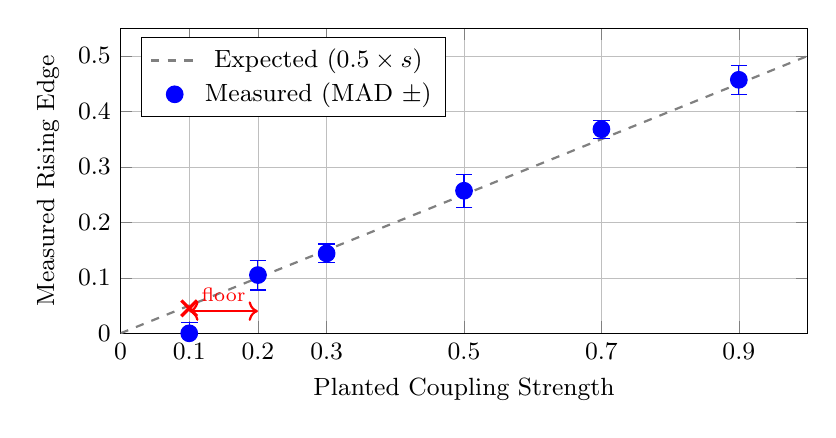
\begin{tikzpicture}
\begin{axis}[
  width=0.85\textwidth,
  height=0.45\textwidth,
  xlabel={Planted Coupling Strength},
  ylabel={Measured Rising Edge},
  xmin=0, xmax=1.0,
  ymin=0, ymax=0.55,
  xtick={0,0.1,0.2,0.3,0.5,0.7,0.9},
  xticklabels={0,0.1,0.2,0.3,0.5,0.7,0.9},
  ytick={0,0.1,0.2,0.3,0.4,0.5},
  grid=both,
  grid style={line width=.1pt, draw=gray!30},
  major grid style={line width=.2pt,draw=gray!50},
  legend pos=north west,
  legend style={font=\small},
  tick label style={font=\small},
  label style={font=\small},
]

% Expected line: y = 0.5 * x
\addplot[domain=0:1, dashed, gray, thick] {0.5*x};
\addlegendentry{Expected ($0.5 \times s$)}

% Measured points
\addplot[only marks, mark=*, mark size=3pt, color=blue,
  error bars/.cd, y dir=both, y explicit]
coordinates {
  (0.1, 0) +- (0,0.019)
  (0.2, 0.105) +- (0,0.027)
  (0.3, 0.144) +- (0,0.017)
  (0.5, 0.257) +- (0,0.030)
  (0.7, 0.368) +- (0,0.016)
  (0.9, 0.457) +- (0,0.026)
};
\addlegendentry{Measured (MAD $\pm$)}

% Detection floor annotation
\draw[<->, red, thick] (axis cs:0.1,0.04) -- (axis cs:0.2,0.04);
\node[red, font=\scriptsize, above] at (axis cs:0.15,0.04) {floor};

% Not detected marker
\addplot[only marks, mark=x, mark size=4pt, color=red, very thick]
coordinates {(0.1, 0.045)};

\end{axis}
\end{tikzpicture}
\caption{Detection sensitivity at noise $\sigma = 0.02$ (linear
coupling). Blue circles: measured rising edge with MAD error bars.
Dashed line: expected edge ($s \times 0.5$). Red $\times$: not
detected (below CFAR threshold). Measurement error consistently
below 5\%. Detection floor lies between coupling 0.1 and 0.2.}
\label{fig:sensitivity}
\end{figure}


\begin{table}[h]
\centering
\caption{Linear coupling strength sweep at noise $\sigma = 0.02$.}
\label{tab:strength}
\begin{tabular}{cccccc}
  \toprule
  Strength & Detected & Rising Edge & Expected & Error & MAD \\
  \midrule
  0.1 & \textbf{no}  & 0.045  & 0.05 & ---  & 0.019 \\
  0.2 & yes          & 0.105  & 0.10 & +5.2\% & 0.027 \\
  0.3 & yes          & 0.144  & 0.15 & $-$4.2\% & 0.017 \\
  0.5 & yes          & 0.257  & 0.25 & +2.9\% & 0.030 \\
  0.7 & yes          & 0.368  & 0.35 & +5.2\% & 0.016 \\
  0.9 & yes          & 0.457  & 0.45 & +1.4\% & 0.026 \\
  \bottomrule
\end{tabular}
\end{table}

The detection floor lies between coupling $0.1$ and $0.2$. At $0.1$,
the planted step amplitude ($0.05$) is comparable to the CFAR
threshold ($k \times \mathrm{MAD} \approx 3.0 \times 0.019 \approx
0.057$). The signal is present but below the noise-adaptive
threshold. Above $0.2$, detection is reliable with measurement error
consistently below $5\%$.

\subsection{Group B: Noise Robustness}

\begin{table}[h]
\centering
\caption{Noise robustness at coupling $s = 0.5$ (expected edge $0.25$).}
\label{tab:noise}
\begin{tabular}{cccccl}
  \toprule
  Noise $\sigma$ & Block & Detected & Edge & MAD & Note \\
  \midrule
  0.01  & 15 & yes & 0.237 & 0.034 & \\
  0.02  & 15 & yes & 0.257 & 0.030 & (Group A cell) \\
  0.05  & 15 & yes & 0.259 & 0.061 & \\
  0.10  & 15 & no  & ---   & 0.124 & signal $<$ threshold \\
  0.10  & 30 & no  & ---   & 0.093 & budget contrast: MAD drops, \\
        &    &     &       &      & still below threshold \\
  0.20  & 15 & no  & ---   & 0.253 & noise equals signal \\
  \bottomrule
\end{tabular}
\end{table}

Detection fails between noise $0.05$ and $0.10$. At noise $0.10$,
the asymptotic CFAR threshold ($k \to 3.0$ as $N \to \infty$) is
$0.30$, permanently above the signal ($0.25$). Doubling the block
size from 15 to 30 reduces MAD by $25\%$ and narrows the gap from
$63\%$ to $14\%$, but does not cross the threshold---the boundary
is governed by the SNR, not the observation budget alone.

\subsection{Group C: False Positives}

\begin{table}[h]
\centering
\caption{False positive test: coupling $s = 0.0$ (no edge exists).}
\label{tab:fpr}
\begin{tabular}{cccc}
  \toprule
  Noise $\sigma$ & Detected & MAD & Trials \\
  \midrule
  0.02  & no & 0.017 & 2 rounds \\
  0.10  & no & 0.116 & 1 round \\
  0.20  & no & 0.136 & 6 rounds \\
  \bottomrule
\end{tabular}
\end{table}

Zero false positives across the full noise range, including extreme
noise ($\sigma = 0.20$) where the MAD is an order of magnitude larger
than at the standard operating point. The threshold is conservative.

\subsection{Group D: Nonlinear Coupling Shapes}

\begin{table}[h]
\centering
\caption{Nonlinear shape generality at noise $\sigma = 0.02$.}
\label{tab:nonlinear}
\begin{tabular}{llcccc}
  \toprule
  Shape & Strength & Detected & Edge & MAD & Note \\
  \midrule
  Saturation  & 0.7 & yes & $-$0.113 & 0.028 & inverted step \\
  Threshold   & 0.7 & yes & \phantom{$-$}0.703 & 0.026 & discontinuous jump \\
  Polynomial  & 0.7 & yes & \phantom{$-$}0.517 & 0.028 & quadratic step \\
  \midrule
  Saturation  & 0.3 & \textbf{no}  & --- & 0.023 & step compressed below floor \\
  Threshold   & 0.3 & yes & \phantom{$-$}0.311 & 0.017 & large step from discontinuity \\
  Polynomial  & 0.3 & \textbf{no}  & --- & 0.005 & step below floor \\
  \bottomrule
\end{tabular}
\end{table}

All three nonlinear shapes are detected at coupling $0.7$.
Saturation produces an inverted step (the response at extreme
parameters is \emph{lower} than at mid-range); the detector
correctly identifies this via the absolute rising-edge test.

At coupling $0.3$, shape matters: threshold coupling is detected
(large step from the discontinuity), but saturation and polynomial
coupling fall below the detection floor. This is expected---nonlinear
shapes compress or redirect the step amplitude, and at low coupling
the compressed signal is indistinguishable from noise.

\section{Discussion}
\label{sec:discussion}

\subsection{What the Protocol Contributes}

The push/pause/hold protocol is the contribution---not the CFAR
detector. CFAR is a well-established technique from radar signal
processing~\citep{finn1968cfar}. What is new is the choreography:
autonomous agents, each with their own objectives and unaware of
each other, take turns as active perturbers and passive observers.
The coordination is minimal---a scheduling constraint (one sender at
a time), not information exchange. Agents do not share objectives,
results, or detected edges.

Without the protocol, there is no signal for CFAR to detect. Two
independently adjusting agents produce confounded objective
trajectories that passive methods cannot separate~\citep{sugihara2012ccm}.
The protocol converts the live system into a sequence of structured
experiments.

\subsection{Detection Boundaries Are Parameterized}

The detection boundaries presented in
Tables~\ref{tab:strength}--\ref{tab:noise} are specific to the
observation parameters listed in Section~\ref{sec:obs-params}. The
method has no fundamental sensitivity limit---the boundary is a
function of observation budget (block sizes, number of rounds) and
detector configuration ($P_{\text{fa}}$, minimum sample counts).
The CFAR scale factor $k$ decreases with more reference cells;
the MAD estimate stabilizes with more samples.

We present results at one operating point ($B = 15$, $P_{\text{fa}} =
0.05$) with one budget contrast ($B = 30$ at noise $0.10$). This
characterizes where the method works and where it stops under
reasonable observation costs. The noise failure at $\sigma = 0.10$
represents an SNR of approximately 2.5:1---an aggressive operating
point for live systems.

\subsection{Threshold Calibration}

The CFAR threshold (\ref{eq:threshold}) is computed from per-sample
noise (MAD of individual objective values), but the detection test
compares block medians. The actual false alarm rate is therefore
lower than the nominal $P_{\text{fa}} = 0.05$---the threshold is
conservative. This is confirmed empirically: zero false positives
were observed across all noise levels (Table~\ref{tab:fpr}). A
median-aware threshold would improve sensitivity at high noise but
requires re-deriving the false alarm rate for median statistics.
We leave this to future work and report results with the conservative
threshold.

\subsection{Nonlinear Coupling}

The protocol is coupling-shape-agnostic by design. The sender pushes
to extreme parameters and returns to neutral; the detector asks
whether the receiver's signal changed and recovered. The shape of
the coupling function determines the step amplitude but not whether
a step exists. All four tested shapes (linear, threshold, saturation,
polynomial) were detected at adequate coupling strength
(Table~\ref{tab:nonlinear}).

At low coupling ($0.3$), nonlinear shapes that compress the step
(saturation, polynomial) fall below the detection floor, while
threshold---which produces a large discontinuous jump---is detected.
This is not a limitation of the protocol but a property of the
specific coupling function's step response at the operating point.

\subsection{Topology Limitation}

The scanner discovers step-change coupling between node pairs. It
does not distinguish direct edges from transitive paths. In a
branching topology (e.g., $A \to B \to D$ and $A \to C \to D$),
node $D$ responds to $A$'s perturbation through transitive paths,
and the scanner would report a step change for the pair $(A, D)$
even though no direct edge exists. Distinguishing direct from
transitive coupling requires either known edge weights to subtract
expected contributions or graph-theoretic analysis on the discovered
step-change graph. This is an open problem for future work.

\subsection{What This Is Not}

This is not causal discovery in the Pearl sense~\citep{pearl2009causality}.
Pearl's framework discovers Boolean causal arrows from interventions
designed by a central researcher. Our agents are not researchers;
they are agents with their own objectives who sacrifice
exploration time to cooperate for measurement. The coordination
is scheduling, not experimental design.

This is also not system identification~\citep{ljung1999sid}, which
requires a specified model structure and estimates parameters within
it. Our method discovers whether coupling exists and measures its
step amplitude, without assuming a model.

\section{Position and Future Work}
\label{sec:position}

\subsection{What This Enables}

Coupling detection is the foundation step of a larger program: building
an empirically-discovered, maintainable coupling model of a live system.
The push/pause/hold protocol produces a coupling scan---a directed graph
of measured step responses between subsystems, valid for the moment it
was taken. This scan is not an end in itself but the basis for:

\paragraph{Characterization.}
The probe data collected during detection already contains more
information than the binary ``coupling detected.'' Each edge carries a
measured step amplitude, a baseline noise level, and a reversibility
fraction. Extracting propagation delay, settling time, and response
curve shape from the same data requires only signal processing---no
additional probing. The scan becomes a characterized connectome:
weighted, directional, per-channel.

\paragraph{Prediction.}
If measured edges compose along graph paths, the coupling graph
becomes a forward model: ``if node $A$ changes by $\Delta$, what is
the predicted response at distant node $D$ through the chain $A \to B
\to C \to D$?'' Whether edges compose linearly or require a learned
composition function is the open question. Chain4 validation (4-node
linear topology, 3 edges) showed measured edges match planted ground
truth---but predicting a distant node's response from composed edges
is not yet tested.

\paragraph{Maintenance.}
A frozen coupling scan serves as a reference model. The system drifts;
the scan ages. Prediction error---comparing the model's expected
response against actual behavior---localizes where structure changed.
This triggers targeted rescanning of the affected neighborhood rather
than a full system rescan. The ratio of scanning to operating adapts
to structural volatility: stable systems need infrequent rescans,
volatile systems need frequent ones.

\paragraph{Cooperation.}
Once agents understand their coupling, they can act on it. Two agents
connected by a coupling edge currently find individually optimal but
jointly suboptimal configurations. The coupling graph reveals
tradeoffs invisible to independent agents. This requires no change to
the detection protocol---only a consumer of the graph it produces.

\subsection{Limitations}

\paragraph{Topology.}
The scanner discovers step-change coupling between node pairs. It does
not distinguish direct edges from transitive paths. In a branching
topology ($A \to B \to D$ and $A \to C \to D$), node $D$ responds to
$A$'s perturbation through transitive paths. The scanner reports a
step change for $(A, D)$ even though no direct edge exists.
Distinguishing direct from transitive coupling is an open problem.

\paragraph{Threshold calibration.}
The CFAR threshold uses per-sample noise (MAD of individual values)
but the detection test compares block medians. The actual false alarm
rate is lower than the nominal $P_{\text{fa}}$---the threshold is
conservative, confirmed empirically by zero false positives across all
noise levels. A median-aware threshold would improve sensitivity but
requires re-deriving the false alarm statistics.

\paragraph{Coordination scale.}
The lease-based turn-taking supports a small number of agents (tested
with 2--4). Scaling to many agents requires group-based coordination
(scoping lease tables by experiment tag) to avoid global contention.
The current global coordination table is a prototype limitation, not
a fundamental constraint.

\paragraph{Auto-calibration.}
Detection parameters---block sizes, push amplitude, cadence,
$P_{\text{fa}}$---are currently fixed. Metaheuristic search could
calibrate these per system, adapting the observation protocol to
each substrate's characteristics. This is future work.

\section{Conclusion}
\label{sec:conclusion}

We presented a push/pause/hold coordination protocol that enables
autonomous agents---unaware of each other, communicating only through
their shared substrate---to discover coupling structure. The protocol
is coupling-shape-agnostic and produces a reversible step signal that
a CFAR detector evaluates against a noise-adaptive threshold.

Empirical validation on a synthetic bench with planted ground truth
shows detection between coupling $0.1$ and $0.2$ at noise $\sigma =
0.02$, with step amplitude measurements within $5\%$ of ground truth.
Zero false positives were observed across all noise levels tested.
All tested nonlinear shapes (saturation, threshold, polynomial) were
detected at adequate coupling.

The coupling scan produced by this protocol is the foundation for a
larger program: characterized connectomes, forward prediction from
composed edges, drift detection through prediction error, and
cooperative agent behavior informed by discovered structure.

\section*{Reproducibility}

All 21 experiment cells (raw detection JSON, observation parameters,
and summary table) and the synthetic bench used to generate them are
available at \url{https://github.com/godon-dev/godon} under
\texttt{papers/detection/}. The coordination protocol
(\texttt{godon-breeders}), CFAR detector (\texttt{godon-causal}), and
bench target (\texttt{godon-bench-generic}) are in separate
repositories within the same organization. All code is open-source
under AGPLv3. Experiments are reproducible via GitHub Actions
workflows that deploy the bench, create agents, run detection rounds,
and query the detector endpoint.


% ── References ────────────────────────────────────────────────────
\bibliography{references}

\end{document}
